\documentclass[20pt, a4paper, oneside, extrafontsizes]{memoir}
\usepackage[utf8]{inputenc} 
\usepackage[T1]{fontenc}
\usepackage{graphicx}
\usepackage[margin=0.3in]{geometry}
\hyphenpenalty 100000
%=============================
\usepackage{datatool}
\DTLloaddb{names}{participants.csv}
\DTLloaddb{instructors}{instructors.csv}
\title{Diplom}



%=============================
\begin{document}
\pagestyle{empty}
%=============================
\DTLforeach{names}{
\name=name}{
%=============================
\begin{figure}[h!]
\centering
 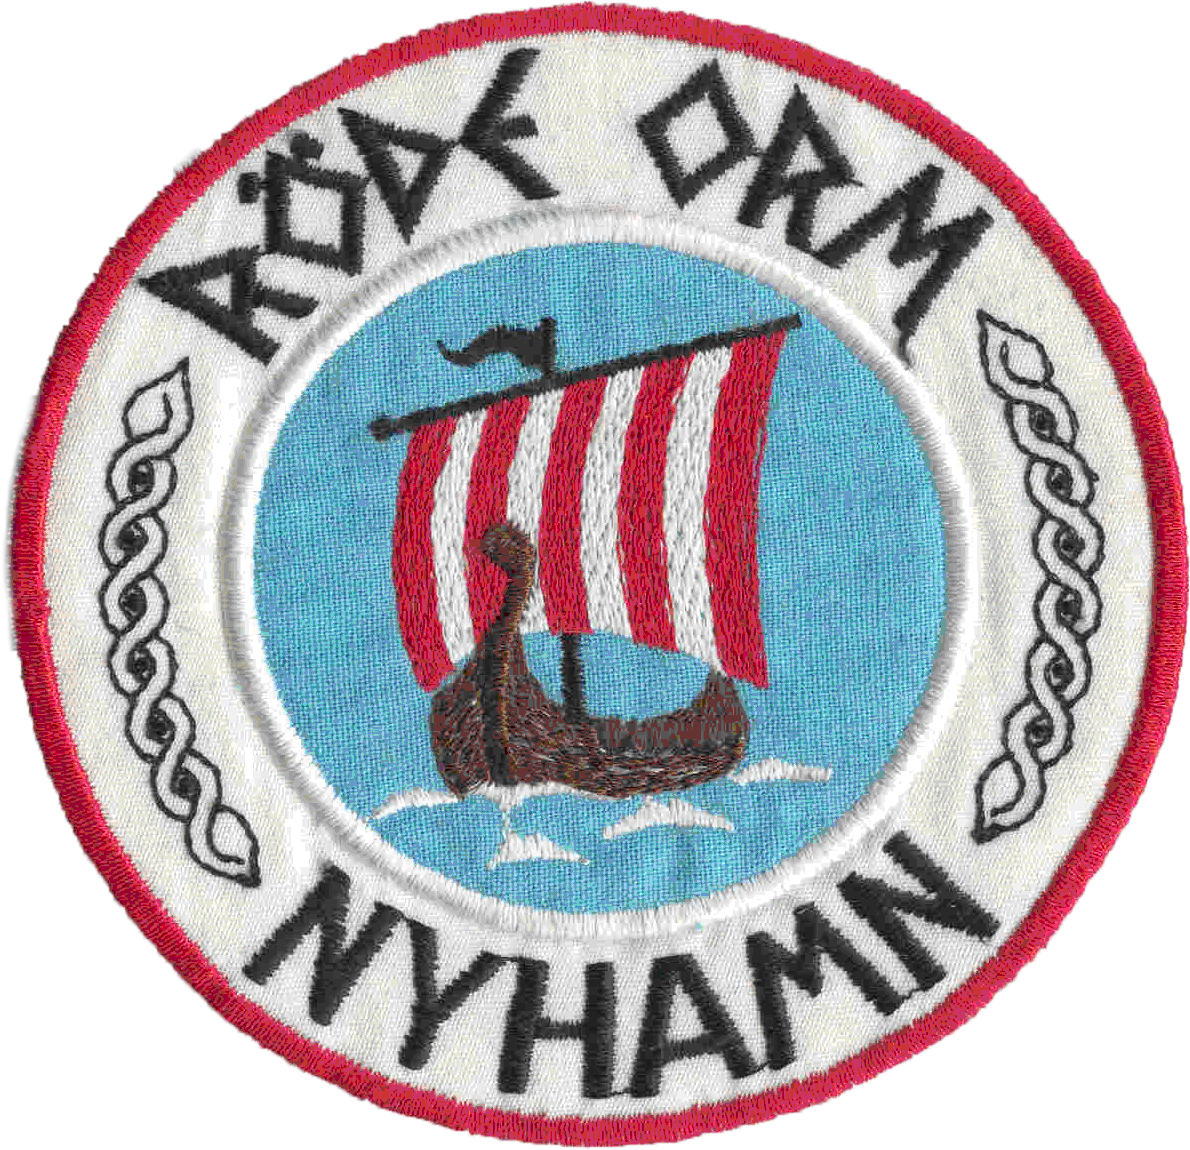
\includegraphics[width=.40\textwidth]{rode-orm-logo}
 \vspace{-1.5em}
\end{figure}
\begin{center}
  \huge{\textbf{\textsc{Diplom}}}
  \vskip0.4em
  \large{till}
  \vskip0.01em
  \Huge{\textbf{\name}}
  \vskip0.4em
  \large{för en väl genomförd}
\end{center}
\begin{figure}[h!]
\vspace{-1.5em}
\centering
 
\includegraphics[width=.75\textwidth]{seglarskola-logo}
 \vspace{-1.5em}
\end{figure}
 \begin{center}
\textbf{Instruktörer}\\
  \DTLforeach{instructors}{\name=name}{
    \name
    \DTLiflastrow{.}{\dtlifnumeq{\DTLcurrentindex}{3}{,\\}{,}}}
    \\
  \textbf{Sommaren \the\year, Nyhamnsläge}
\end{center}

%=============================
\pagebreak
}
\end{document} 
